\chapter{Roadmap Methods for Motion Planning}
\label{chap:roadmaps}

Robots are fundamentally agents that move through the world,
and so the question of how to best deliberate about motion
is a central problem in robotics.
Different tasks and problem domains expose a vast array of
qualities and properties of motion that are important
-- for example, motion that is expressive, efficient, or expected
-- and algorithms can rely on a rich and growing set
of models and methodologies in order to generate such motion.

Underlying this rich tapestry of robotic motion
is the most fundamental abstraction of motion planning --
finding a path for a system which accomplishes a motion task
without colliding with obstacles.
While this might at first seem straightfoward,
finding such paths for articulated robotics in
complex semi-structured environments
is no easy feat,
and finding such paths quickly and efficiently
is of upmost important.

This chapter includes a brief introduction to
the motion planning problem.
Due to its paramount importance to robotics,
variations on this problem have deservedly
enjoyed a considerable amount of attention over the past 40 years.
We tailor our investigation towards aspects of the problem
that are relevant to this thesis.
In particular,
we provide an overview of a class of approaches called roadmap methods
that are well-suited to motion planning for articulated robots.
For a comprehensive treatment,
we refer to LaValle \citep{lavalle2006planningbook}.

\section{The Motion Planning Problem}

\begin{marginfigure}
   \centering
   \includegraphics{build/movers-problem-schwartz-sharir} %
   \caption{The original mover's problem
      \citep{schwartzsharir1983pianomovers1}
      entails finding a collision-free path for a geometric body
      amongst obstacles,
      or finding that no path exists.}
   \label{fig:roadmaps:movers}
\end{marginfigure}

The earliest instances of motion planning considered a single rigid
body moving within a geometric environment consisting of
fixed obstacles
(Figure~\ref{fig:roadmaps:movers}).
Termed the \emph{FindPath} or \emph{piano mover's} problem,
this representation and variations thereof were extensively studied
\citep{lozanoperezwedley1979collisionfree,
   schwartzsharir1983pianomovers1},
for various dimensionalities (e.g. two or three)
and obstacle representations (e.g. polygonal regions).
Importantly,
these earlest problems exhibited two fundamental properties
inherent in all motion planning problems:
(a) that solutions, called \emph{paths}, are continuous, and
(b) that the objective is binary, with any
prospective path either in collision or collision-free.
The problem entails finding a non-colliding path if one exists,
or returning with failure otherwise.

\begin{marginfigure}
   \centering
   \includegraphics{build/c-space} %
   \caption{The motion planning problem entails finding a continuous
      path among obstacles in an abstract configuration space.}
   \label{fig:roadmaps:cspace}
\end{marginfigure}

A generalization of the piano over's problem
commonly called the \emph{motion planning problem}
entails an abstraction of the single rigid body
to an arbitrary \emph{configuration space} (C-space)
\citep{lozanoperez1983cspace}.
Any point $q$ in this abstract space $\mathcal{C}$
(see Figure~\ref{fig:roadmaps:cspace}),
corresponds to a full configuration of the system,
such has the position and orientation of a rigid body.
Importantly,
$\mathcal{C}$ can also capture the full configuration (or joint)
space of an articulated robotic manipulator.

Any point $q \in \mathcal{C}$ corresponds to a particular geometric
configuration of the robot within its fixed environment.
If this configuration entails a geometric collision in the workspace
(either between the robot and the environment,
or the robot with itself),
this point lies within a \emph{configuration-space obstacle}.
The union of these configurations comprises the set of obstacle
configurations $\mathcal{C}_{\ms{obs}}$.
Collision-free configurations and paths must be contained entirely
in the complement of this set,
$\mathcal{C}_{\ms{free}} = \mathcal{C} \setminus \mathcal{C}_{\ms{obs}}$.

A path $\xi : [0,1] \rightarrow \mathcal{C}$
is called collision-free if
$\xi(t) \in \mathcal{C}_{\ms{free}} \;\forall t \in [0,1]$.
A continuous path $\xi$ satisfies a particular motion planning query
with start and goal configurations $q_{\ms{start}}$ and $q_{\ms{goal}}$
if $\xi(0) = q_{\ms{start}}$ and $\xi(1) = q_{\ms{goal}}$.

\subsection{Optimal Motion Planning}

The optimal motion planning problem is a generalization which
includes a metric over solution paths
$x : \Xi \rightarrow \mathbb{R}$.
See \citep{karaman2011samplingoptimal}.

\subsection{Further Generalizations}

\cdnote{
There are other generalizations such as kinodynamic planning.
Here, a solution is commonly called a trajectory.
Optimal variants may have costs on the actions as well.
Intro: focus on configuration-space planning (not kinodynamic planning).
What about constraints? We won't deal with these much either.
}

\section{Motion Planning by Discretizing C-Space}

We give a brief review of approaches to motion planning that rely
on discretizations of the configuration space.

\subsection{Building Graphs in C-Space}

The formulation of motion planning via the configuration space
raises the question:
how can we test whether a motion is collision-free?
This question is especially delicate when the geometry is complex
and the configuration-space obstacles cannot be represented explicitly.
In this case,
it is necessary to test prospective configurations and motions
for membership in $\mathcal{C}_{\ms{free}}$ using indicator functions.
\begin{equation}
   \mathbf{1}_{\mathcal{C}\ms{free}} : \mathcal{C} \rightarrow \{ \mbox{True}, \mbox{False} \} 
   \mbox{\quad s.t. \quad}
   \mathbf{1}_{\mathcal{C}\ms{free}}(q) = 1 \mbox{ iff } q \in \mathcal{C}_{\ms{free}}.
\end{equation}
Note that implementing $\mathbf{1}_{\mathcal{C}\ms{free}}$ for an articulated robot
entails computing the forward kinematics of the robot at the
query configuration,
and running a collision check in the workspace.

We can rely on the functional variant to test a path $\xi$:
\begin{equation}
   \mathbf{1}_{\Xi\ms{free}} : \Xi \rightarrow
      \{ \mbox{True}, \mbox{False} \} 
\end{equation}
Talk about committing to a resolution to test with,
which is what we do in this thesis.
Note that this is only an approximation.
You should pad your obstacles so you don't plan through wires.
But also link to C-space bubble stuff
\citep{quinlan1994modification}.

\paragraph{Composing Motions.}
Importantly,
two paths $\xi_{ab}$ and $\xi{bc}$ with $\xi_{ab}(1) = \xi_{bc}(0)$
can be concatenated to a path $\xi{ac}$,
with
\begin{equation}
   \mathbf{1}_{\Xi\ms{free}}(\xi_{ab})
   \;\cap\;
   \mathbf{1}_{\Xi\ms{free}}(\xi_{bc})
   \iff
   \mathbf{1}_{\Xi\ms{free}}(\xi_{ac}).
\end{equation}
This motivates approaches which maintain a graph structure of
smaller valid motions in the configuration space.
Consider a graph $G = (V,E)$,
with each vertex $v \in V$ a configuration $q \in \mathcal{C}$
and each edge $e \in E$ a path $\xi$
s.t.  $\mathbf{1}_{\Xi\ms{free}}(\xi) = \mbox{True}$.
If $v_{\ms{start}}, v_{\ms{goal}} \in V$
correspond to the query vertices $q_{\ms{start}}, q_{\ms{goal}}$,
then a path $p$ through $G$ from
$v_{\ms{start}}$ to $v_{\ms{goal}}$
corresponds to a collision-free solution to the motion planning problem.

The approach for constructing, searching, and validating this graph
differs significantly between algorithms.
We will broadly review different options in
Section~\ref{sec:roadmaps:sensitivity}.

\begin{marginfigure}
   \centering
   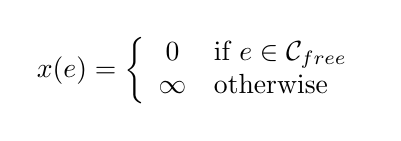
\begin{tikzpicture}
      \node at (0,0) {
         $x(e) = \left\{ \begin{array}{cl}
            0 & \mbox{if } e \in \mathcal{C}_{\ms{free}} \\
            \infty & \mbox{otherwise} \\
         \end{array} \right.$
      };
   \end{tikzpicture}
   \caption{Edge cost model
      for the (feasible) motion planning problem.}
\end{marginfigure}

\begin{marginfigure}
   \centering
   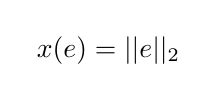
\begin{tikzpicture}
      \node at (0,0) {
         $x(e) = || e ||_2$
      };
   \end{tikzpicture}
   \caption{$L_2$-norm edge cost model
      for the optimal motion planning problem.}
\end{marginfigure}

\cdnote{Talk about execution costs that are additive!}

%\paragraph{Resolution and Probabalistic Completeness.}
%Any discretization is only an approximation of the actual configuration
%space.
%Of course, the discretization is always just an approximation
%of the actual C-space.
%Hopefully, you can choose a discretization strategy that allows your
%algorithm to have one or both of these forms of completeness.

\paragraph{Motion Planning as Pathfinding.}
\label{subsec:roadmaps:planning-as-pathfinding}
Here, talk about how even if there are multiple available
start or goal configurations
(e.g. different grasps or inverse kinematics solutions),
the motion planning problem can still be posed as a
single-pair shortest path (SPSP) problem
by augmenting the graph with virtual source sink vertices
and edges.

\paragraph{Other Approaches to Motion Planning.}
The motion planning problem affords a number of different classes of
algorithms.
One such class which is especially well-suited to easier instances
is trajectory optimization.
Approaches such as CHOMP \citep{zucker2013chomp}
and TrajOpt \citep{schulman2013trajopt})
commit to a trajectory representation for $\xi^{(1)}$
and use require stronger world descriptions
(SDFs, convex obstacle decompositions)
to make local modifications
to produce a new path $\xi^{(2)}$.
Also,
optimizers are commonly used in lower levels to react to local
changes (e.g. \citep{quinlan1994modification}).

\section{Obstacle Sensitivity}
\label{sec:roadmaps:sensitivity}

Generally,
graph-based motion planners require the following three stages:
(a) constructing the graph,
(b) searching the graph, and
(c) validating the graph.

One of the key differentiators between graph-building techniques
for motion planning available in the literature
is how they interleave constructing, searching, and validating
the graph.
This section reviews one important consideration:
the degree of dependence of the graph structure
on the distribution of obstacles in the scene.
We broadly categorize algorithms into two groups:
those that are \emph{obstacle-sensitive},
and those that are \emph{obstacle-insensitive}.

\subsection{Obstacle-Sensitive Approaches}
\label{subsec:roadmaps:sensitive}

In obstacle sensitive approach,
the graph is built incrementally,
and construction of new elements
is directly interleaved with validating them,
in response to the distribution of valid or costly states.

\paragraph{Exact Algorithms.}
The earliest work on the motion planning problem studied exact
algorithms which worked directly on an explicit representation
of the obstacles (e.g. polygons) \citep{lozanoperez1983cspace}.
These approaches can guarantee optimal solutions,
and don't require edge validation if implemented correctly.
However,
they are difficult to apply to problems on articulated
robots for two reasons.
First, many are only applicable to problems in two or three dimensions.
Second, an explicit representation of obstacles in the
configuration space is exceedingly difficult due to the
nonlinearity in the forward kinematics function.

\paragraph{Treebuilding Algorithms.}
Other approaches treat the configuration space implicitly.
The most common algorithms grow and validate trees simulteneously,
either unidirectionally or bidirectionally.
At each iterations,
these algorithms use a sampling strategy to propose a new extension,
and then augment their tree(s) if the new motion is found to be valid.

Key examples of this approach include
Expansive Space Trees (EST) \citep{hsu1997expansive}
and Rapidly-exploring Random Trees (RRT)
\citep{lavalle1998rrt, kuffner2000rrtconnect}.
SBL \citep{sanchezante2001sbl}
is a bidirectional EST with lazy edge validity checking.

\paragraph{Planning vs. Execution Cost.}
The core algorithms in this category are primarily feasibility
algorithms;
there is no mechanism explicitly biasing them to select
low-cost paths.
\marginnote{We talk about this tradeoff in detail
in Chapter~\ref{chap:lemur}.}
Therefore, solutions found tend to be of low quality,
and they are customarily optimized using a path shortcutting
algorithm.
More recent work has also focused on asymptotically optimal variants
of these planners \citep{karaman2010rrtstar}.

\paragraph{Advantages of Obstacle Sensitivity.}
One key advantage to obstacle-sensative approaches is that
they only construct the graph structure in the parts of the
configuration space that are relevant to the planning query.
The Vornoi bais of the RRT or the importance sampling of the EST
attempt to focus sampling graph construction in ares
which tend to improve the current solution.

Another advantage is that these algorithms handle densification
naturally;
the graph structure is augmented automatically,
so the resolution of the discretization need not be explicitly
increased as the instance reveals to be more difficult.

%It's important to compare against these.
%But we focus on insensitive approaches.

\cdnote{Visibility PRMs \citep{simeon2000visibilityprms}.}

%Usually, densification comes for free.

%Probabalistic completeness.

\subsection{Obstacle-Insensitive Approaches}

In contrast to the obstacle-sensitive approaches described in
Section~\ref{subsec:roadmaps:sensitive},
the approaches in this section commit to a particular discretization
of the configuration space a priori,
independent of the distribution of obstacles or costs.
While this simpler method forgoes some of the advantages of
obstacle sensitivity,
this idependence does confer some advantages of its own.

\paragraph{Roadmap Methods.}

The earliest obstacle-insensitive methods particular to the motion
planning problem are called \emph{roadmap methods}.
The term roadmap usually connotes a graph embedded in a continous
ambient space in the presence of obstacles.
Vertices in the graph are also called milestones.
The first roadmap methods such as the
Probabalistic RoadMap (PRM) \citep{kavrakietal1996prm}
initialized the milestones arrangement
from a uniform distribution over the free space.

Key to sampling-based approaches
to motion planning for such problems
is the concept of the \emph{local planner}.
Given two configurations $q_a, q_b \in \mathcal{C}$,
the local planner first produces a candidate path $\xi_{ab}$ between
them.
(A common implementation simply produces the straight-line path
in configuration space.)
Edges are only attempted when they meet certain restrictions.

There are some variants of roadmap planners that are not independent
of the obstacle distribution.
First,
many roadmap planners make use of a heuristic ``expansion'' step
wherein additional samples are added to the roadmap
in order to increase its connectivity.
Second,
edge connection rules that can forgo connections within
the same connected component.

%\cdnote{Densification?}

\paragraph{Search-based Methods.}
Graph pathfinding algorithms such as A* \citep{hart1968astar}
are applicable to the motion planning problem if a suitable
space discretization is considered.
The search space is often represented implicitly via a set of
operators or motion primitives
which reproduce a regular lattice over the configuration space
\citep{pivtoraiko2005statelattice};
when the lattice is rectangular,
seach-based planning is also called ``grid search.''

\paragraph{Lazy Validity Checking.}
Because obstacle-insensitive approaches decouple graph construction
from validity checking,
it is often advantageous to defer the latter until it is
necessary for solving the query at hand.
Lazy validity checking has been exploited
in roadmap methods such as the Lazy PRM
\citep{bohlin2000lazyprm, hauser2015lazy},
search methods such as Lazy Weighted A* \citep{cohen2014narms},
and methods which bridge the two such as FMT* \citep{janson2015fmtstar}.
We discuss laziness in graph search comprehensively
in Chapter~\ref{chap:lazysp}

\paragraph{Adaptive Densification.}
One difficulty with these obstacle-insensitive approaches
is that they commit to a particular discretization,
and once their search is exhausted,
they must return the best path found,
or nothing if no path was found so far.
This property is known as resolution completeness
\citep{cheng2004rescomplete}.
Algorithms such as BIT* \citep{gammell2015bitstar}
consider a sequence of progressively densified approximations
in order to produce an anytime sequence of improving solution paths.

\begin{figure}
   \centering
   \includegraphics{build/roadmap-stack}
   \caption{Roadmap stack.}
\end{figure}

\paragraph{Advantages of Obstacle Insensitivity.}
The obstacle sensitivity question represents an underlying efficiency
tradeoff.
Sensitive approaches may be able to adapt their discretization more
directly to local obstacle distributions.
On the other hand,
insensitivity to obstacles admits a number of efficiency advantages.
Much of the nearest-neighbor computation
often required during graph construction can be cached and amortized
over all planning queries.
Other properties of the discretization that are constant between
similar planning instances can also be shared
as described in Chapter~\ref{chap:family}.
For these reasons,
this thesis build on top of obstacle-insensitive roadmaps.

\section{Roadmap Classes}

Roadmap methods operate over a graph constructed in the
robot's configuration space.
Roadmap miletones are commonly genererated by a number of different
types of point sequences,
and edges are considered between vertices pairs that meet
certain constraints.
While most algorithms methods are generally agnostic
to the class of roadmap that they operate on,
choosing a suitable class and its parameters has a large effect
on both theoretical and practical perforamce.

\paragraph{Random Sequences.}
The original roadmap algorithms
\citep{kavrakietal1996prm}
operated primarily over sets
of vertices drawn uniformly at random from the configuration space.
Many more recent algorithms such as
RRT* \citep{karaman2010rrtstar},
PRM* \citep{karaman2011samplingoptimal},
FMT* \citep{janson2015fmtstar},
and BIT* \citep{gammell2015bitstar} make use of the same
uniform obstacle distribution.
Such a distribution is attractive both because
it is simple to implement
it because it allows for theoretical properties such as
completeness and optimality to be demonstrated
in probability.

\paragraph{Deterministic Sequences.}
Many researchers have examined whether randomness is a necessary
(or even beneficial) aspect of treebuilding and roadmap planners
\citep{branicky2002detvsprobroadmaps}.
This is especially relevant in the context of comparing
roadmap planners with search-based methods
that conventionally operate over lattices \citep{lavalle2002gridprms}.

One of the most straightforward disadvantages of using a
non-deterministic sequence for each motion planning query
is that the constructed graph is different for each query.
This makes it impractical to pre-compute and amortize nearest
neighbor queries across problem instances,
as well as to pre-compute edge states as decribed in
Chapter~\ref{chap:family}.

Further,
theoretical properties of roadmap methods
such as resolution completeness and asymptotic optimality
depend on properties of the underlying point set
such as its \emph{dispersion}.
Not only can the dispersion of a set of randomly sampled points
only be established in expectation,
but it is demonstrably larger than the dispersion of other
well-known point sequences,
such as the Halton or Hammersley set,
or the Sukharev grid.
For an in-depth analysis of differet point sets for roadmap
planning, see Janson \citep{janson2015deterministicsampling}.

\begin{figure}
   \centering
   \includegraphics{build/roadmaps/gen/aagrid}
   \includegraphics{build/roadmaps/gen/rgg}
   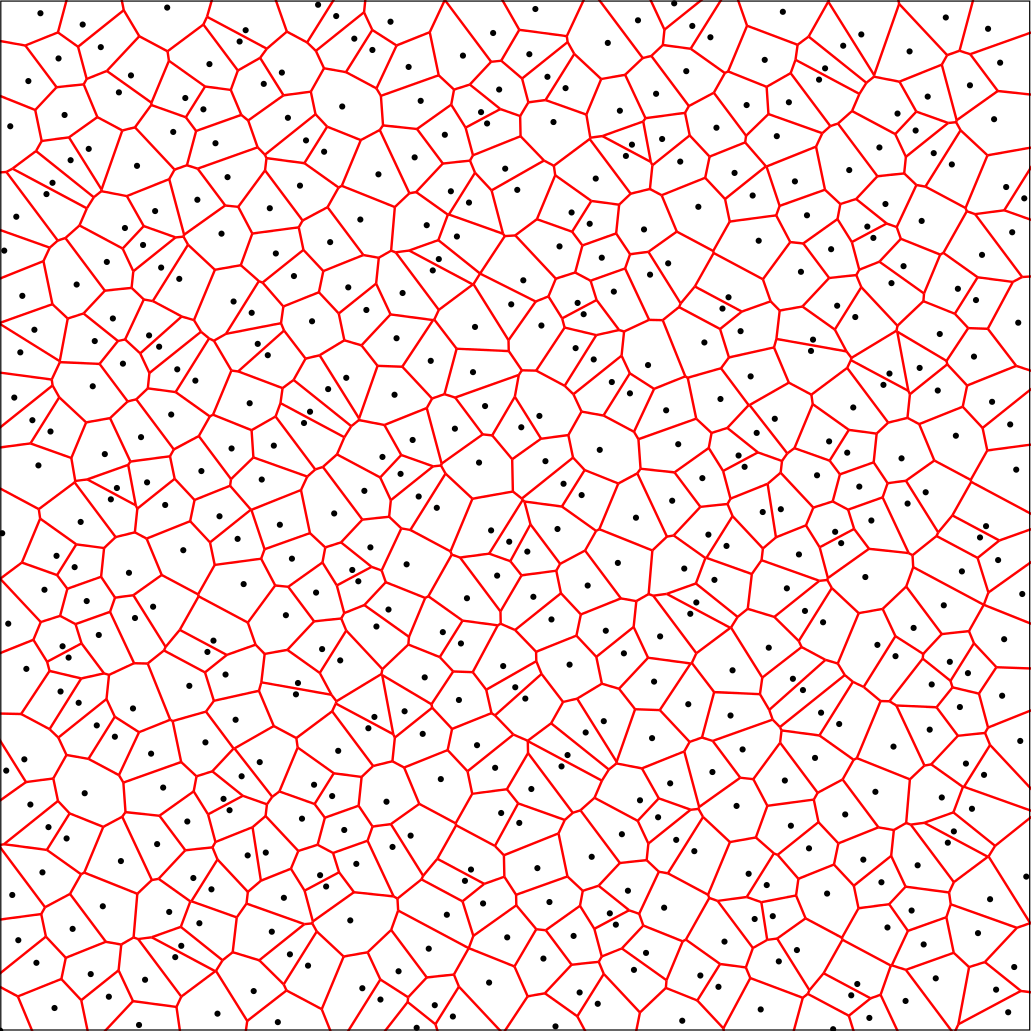
\includegraphics{build/roadmaps/gen/halton}
   \caption{Examples of roadmap types over the unit square
      (axis-aligned lattice, RGG, and Halton graphs).
      In this case, all roadmaps have a connection radius of 0.3.}
\end{figure}

\paragraph{Connection Radii.}
Previous work \citep{karaman2011samplingoptimal} has established
that a roadmap planner which uses a uniformly randomly generated
point set is asymptotically optimal almost surely
if if the edge connection radius $r$ is sufficiently large w.r.t.
the number the number of samples $n$.
In particular,
it defines the critical value $\gamma^*_{\mathcal{C}}$:
\begin{equation}
   \gamma^*_{\mathcal{C}}
      = 2 \left( \left[ 1 + \frac{1}{d} \right]
         \frac{\lambda_d(\mathcal{C})}{\zeta_d} \right)^{1/d},
\end{equation}
where $d$ is the dimensionality of the configuration space,
$\lambda_d(\cdot)$ represents the Lebesgue measure (e.g. volume),
and $\zeta_d$ is the Lebesgue measure of the $d$-dimensional unit ball.

Asymptotically optimal under uniform sampling requires
an edge connection radius $r_{\ms{log}}$:
\begin{equation}
   r_{\ms{log}}(n) =  \gamma^*_{\mathcal{C}} \, \eta
      \left( \frac{\log(n)}{n} \right)^{1/d}
\end{equation}
for some tuning parameter $\eta > 1$.
Point sets with tighter dispersion bounds,
such as the Halton sequence,
can exploit a smaller connection radius $r_{\ms{log}}$:
\begin{equation}
   r_{\ms{loglog}}(n) = \gamma_{\mathcal{C}} \, \eta
      \left( \frac{\log(\log(n))}{n} \right)^{1/d}.
\end{equation}
For details we refer the reader
to \citep{janson2015deterministicsampling}.

\paragraph{Roadmaps for Articulated Robots.}
We apply roadmap methods to the three robot platforms
from Chapter~\ref{chap:intro} in this thesis.
Unless otherwise noted,
we build roadmaps directly in the joint space of the robot.
See Table~\ref{table:roadmap-params} for the roadmap parameters
that we use.

\begin{table}
   \centering
   \begin{tabular}{lccc}
      \toprule
      & HERB & CHIMP & IRB4400 \\
      \midrule
      $d$ & 7 & 7 & 6 \\
      $\gamma^*_{\mathcal{C}}$ & 7.67 & 7.97 & 7.74 \\
      $r_{\ms{log}}$ & 2.83 & 2.93 & 2.41 \\
      $r_{\ms{loglog}}$ & 2.31 & 2.40 & 1.90 \\
      \bottomrule
   \end{tabular}
   \caption{Table of roadmap connection radii parameters for
      various scaling rates across the different robot platforms
      considered in this thesis.
      Radii presented are for $n=10000$ and $\eta = 1$
      and are given in radians.}
   \label{table:roadmap-params}
\end{table}

%\subsection{Dispersion}
%
%Deterministic sampling and dispersion:
%\citep{janson2015deterministicsampling}.
%
%\begin{figure}
%   \centering
%   \includegraphics{build/roadmaps-dispersion/dispersion}
%   \caption{Dispersion plot on the unit square.
%      Green is the dispersion of an incremental (greedy) Sukharev
%      grid.}
%\end{figure}
%
%\begin{figure}
%   \centering
%   \includegraphics{build/roadmaps-dispersion/dispersion-herb}
%   \caption{HERB dispersion plot.}
%\end{figure}
%
%\begin{figure}
%   \centering
%   \includegraphics{build/roadmaps-dispersion/dispersion-irb4400}
%   \caption{IRB4400 dispersion plot.}
%\end{figure}

%\subsection{Batch Size}
%
%\begin{figure}
%   \centering
%   \begin{tikzpicture}
%   \begin{axis}[
%         xmode=log,
%         xlabel={Batch Size},
%         ylabel={LazySP Time (s)},
%         xlabel near ticks,
%         ylabel near ticks,
%         ]
%      \addplot coordinates {
%         (100, 0.2407595708)
%         (250, 0.27367886569999994)
%         (1000, 0.2165730066)
%         (2500, 0.3836524094)
%         (10000, 0.47772694290000006)
%      };
%   \end{axis}
%   \end{tikzpicture}
%   \caption{Batch size. {\tt herbbin0}, seeds 1-10, gammafac=1, lambda=0.}
%\end{figure}
